\documentclass[11pt]{article}

\usepackage[left=0.75in, right=0.75in, top=0.75in, bottom=0.75in]{geometry}
\usepackage{layout}
\usepackage{ucs}
\usepackage[utf8x]{inputenc}
\usepackage{titlesec}
\usepackage{graphicx}
\usepackage{amssymb}
\usepackage{amsmath}
\usepackage{dsfont}
\usepackage{float}
\usepackage{caption}
\usepackage{subcaption}
\usepackage{array}
\usepackage[]{mcode}

\title{\textbf{TS 214 - TP}\\Compression/Décompression d'une image binaire}
\author{Maxime PETERLIN - \texttt{maxime.peterlin@enseirb-matmeca.fr}\\
Gabriel VERMEULEN - \texttt{gabriel@vermeulen.email} \\\\{ENSEIRB-MATMECA, Bordeaux}}
\date{18 décembre 2014}


\begin{document}

\maketitle
\tableofcontents

\newpage

\section{Introduction}

	Le but de ce TP est d'établir une chaîne de compression et de décompression, afin de l'appliquer sur des images binaires. Ces algorithmes sont basés sur les technologies de compression utilisées par les fax. La compression se fait sans perte et est basée sur un codage de Huffman modifié (MH) particulièrement adapté aux images monochromes. Ce codage s'effectue ligne par ligne.\\
	Ce rapport commencera par l’explication d'une méthode de compression et de décompression, puis détaillera l'implémentation de cette dernière sous MATLAB et enfin présentera les résultats obtenus.

\section{Méthode de compression et de décompression}

	\subsection{Codage d'une page}
	
	Le codage d'une page s'effectue en plusieurs étapes. Chaque lignes est traitées indépendamment des autres. L'image étant binaire, elle est composée uniquement de $0$ et de $1$. Un pixel noir correspondant au bit $0$ et un pixel blanc au bit $1$.\\
	La première étape pour encoder une ligne consiste à déterminer la longueur des séquences successives de pixels noir et blancs. Le codage commence toujours par une longueur de séquence blanche, qui peut donc être nulle si le premier pixel est noir.\\
	Ensuite ces données sont encodées en fonction de deux tables prédéfinies, une pour les séquences de pixels blancs et une pour les séquences de pixels noirs. Si la longueur de séquence est inférieur à $64$, elle est directement encoder. Sinon il faut concaténer deux informations : la première, appelé MakeUp, est l'encodage d'un nombre multiple de $64$, la deuxième, appelé Terminating, est l'encodage d'un nombre compris entre $0$ et $63$. Ainsi pour encoder un nombre supérieur ou égale à $64$, il faut encoder le multiple le plus proche de $64$ par valeur inférieure et ensuite encoder le nombre résultant de la différence du nombre qu'on souhaite encode avec le multiple choisi.\\
	Enfin pour terminer une ligne, on y ajoute le code EOL (End-Of-Line) : $000000000001$\\\\
	Une fois que toutes les lignes ont été codées, on y ajoute une ligne contenant six fois le code EOL. Cela traduit la fin d'une page.
	
	\subsection{Décodage d'une page}
	
	La méthode retenue pour décoder une page est basée sur l'un des principes du codage de Huffman : un code ne peut pas être le préfixe d'un autre. On représente ainsi les codes sous la forme de deux arbres, l'un pour les codes de séquences de pixels blancs et l'autre pour les codes de séquences de pixels noirs. Il est alors possible de décoder ces séquences en parcourant ces arbres et de récupérer les pixels de l'image.

\section{Implémentation MATLAB}
	
	\subsection{Codage d'une page}
	
	La première fonction créée permet de calculer la longueur des séquences de pixels blancs et noirs. Cela se fait en une ligne :
	\begin{lstlisting}
		ligne_out = diff([ 0 find(diff(ligne_in)) length(ligne_in)]);
	\end{lstlisting}

	Si le premier pixel est noir, il faut ajouter une séquence nulle de pixels blancs et on obtient ainsi la séquence binaire qu'il faut encoder :
	\begin{lstlisting}
		ligne_out = [0 ligne_out];
	\end{lstlisting}
	
	Il faut ensuite importer les fichiers $black\_codes.txt$ et $white\_codes.txt$. Cela se fait grâce à notre fonction $input\_file()$ :
	\begin{lstlisting}
		function [ data ] = input_file( filepath )
			a = fopen(filepath, 'r');
			data = [];
			while(~feof(a)) % Tant qu'il y a des choses a lire
				b = fgetl(a); % On recupere une ligne
				c = strsplit(b, '\t'); % On separe les deux elements
				data = [data; c];
			end
			fclose(a);
		end
	\end{lstlisting}
	
	On peut maintenant encoder notre ligne. Pour se faire nous avons créé une fonction $code\_ligne()$ (voir annexe).\\
	Afin de coder les données en uint8, il a fallut effectuer un padding à $0$, c'est-à-dire ajouter des bits $0$ à la fin de la ligne pour que la longueur totale de la ligne soit multiple de 8.
	
	Enfin, pour sauvegarder le résultats du codage de la ligne, nous ecrivons les données dans une fichier grâce aux fonctions $fopen()$ et $fwrite()$.
	
	\subsection{Décodage d'une page}
	
	Pour décoder une page, il faut commencer par récupéré une ligne dans un fichier, ce qui se fait avec les fonctions $fopen()$ et $fgetl()$.\\
	Les arbres permettant le décodage étant fourni, il a fallu créer une fonction qui parcoure ces arbres en fonction des données récupérées par la lecture du fichier. Cette fonction est nommée $decode\_doc()$ (voir Annexes).\\
	Cette fonction retourne un ensemble de vecteurs contenant chacun les longueurs de séquences de pixels noirs et blancs correspondant à chaque ligne.\\
	Afin de reconstruire l'image, une fonction nommée $reconstruction()$ a été implémenté. Elle retour l'image binaire à partir de l'ensemble de vecteurs décrit précédemment.

\section{Application et résultats}
	
	\subsection{Compression}
	
	Le but de cette application est d'encoder et de décoder cette image :
	
		\begin{figure}[H]
			\centering
			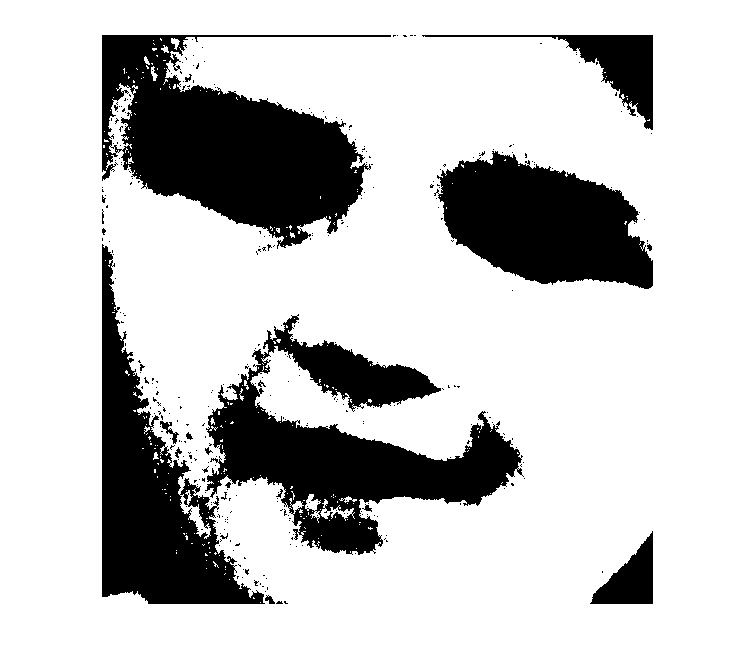
\includegraphics[scale=0.6]{img/img_ori.png}
			\caption{Image à encoder}
			\label{img1}
		\end{figure}
	
	Après encodage, voici le résultats de compression obtenue :\\
		- Taille de l'image brute : 39 190 octets.\\
		- Taille de l'image compressée : 8 722 octets.\\
	Le taux de compression est égale à $4,49$.
	
	\subsection{Décompression}
	
	Après décodage on obtient l'image suivante :

		\begin{figure}[H]
			\centering
			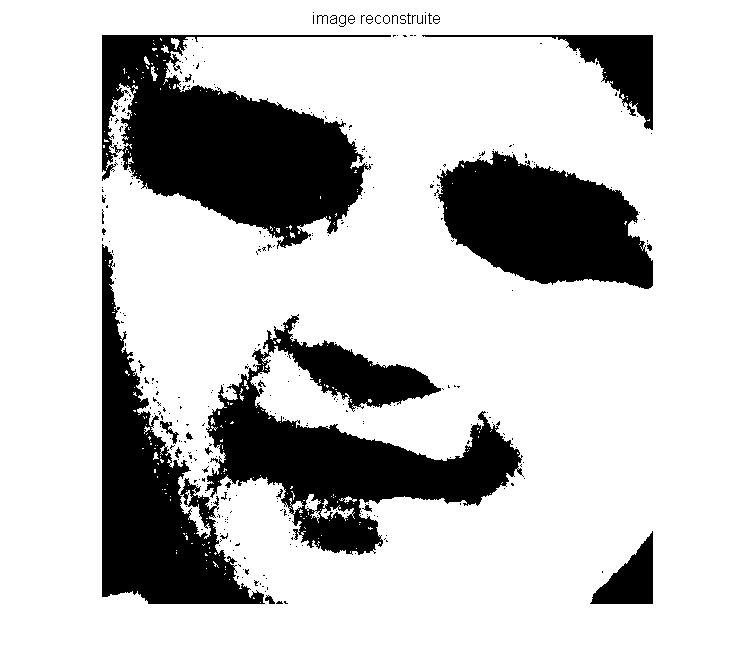
\includegraphics[scale=0.6]{img/img_dec.png}
			\caption{Image décompressée}
			\label{img2}
		\end{figure}
		
		Le taux d'erreur est nul ce qui montre que la compression s'est effectuée sans perte.
	
	\subsection{Comparaison des résultats}
	
	La comparaison s'effectue grâce à la fonction $imwrite()$ qui permet de compression directement une image en $FAX3$ et en $FAX4$.
	
	\begin{lstlisting}
		imwrite(img_origine, 'img_fax3.tif', 'Compression', 'fax3');
		imwrite(img_origine, 'img_fax4.tif', 'Compression', 'fax4');
	\end{lstlisting}
	
	- Taille de l'image d'origine : 39 190 octets.\\
	- Taille de l'image compressée : 8 722 octets.\\
	- Taille de l'image compressée par $FAX3$ : 7 842 octets.\\
	- Taille de l'image compressée par $FAX4$ : 5 596 octets.\\
	
	La méthode de compression mise en place n'est donc pas la plus performante mais compression relativement bien une image.

\section{Conclusion}

	Ce TP nous aura permit de mettre en pratique nos connaissances théoriques de la compression et décompression de données. Il intéressent de voir qu'il est possible de compresser avec un ratio supérieur à 4 une image binaire sans aucune perte.

\section{Annexes}

	\begin{lstlisting}
		function [ line_out ] = code_line ( line_in, white, black )
    s = 0; % variable pour changer du blanc au noir et vis versa
    line_out = '';
    for i=1:length(line_in)
        v = line_in(i);
        if(v >= 64)
            code = fix(v/64)*64;
            rest = v - code;
            if(s == 0)
                [~, id1] = ismember(int2str(code), white);
                [~, id2] = ismember(int2str(rest), white);
                line_out = strcat(line_out, white{id1, 2}, white{id2, 2});
                s = 1;
            else
                [~, id1] = ismember(int2str(code), black);
                [~, id2] = ismember(int2str(rest), black);
                line_out = strcat(line_out, black{id1, 2}, black{id2, 2});
                s = 0;
            end
        else % < 64
            if(s == 0)
                [~, id1] = ismember(int2str(v), white);
                line_out = strcat(line_out, white{id1, 2});
                s = 1;
            else
                [~, id1] = ismember(int2str(v), black);
                line_out = strcat(line_out, black{id1, 2});
                s = 0;
            end
        end
    end
    % Ajout de EOL
    line_out = strcat(line_out, '000000000001');
    
    % Padding
    l = length(line_out);
    nb_padding = fix(l/8 + 1)*8 - l;
    padding = strrep(int2str(zeros(1, nb_padding)), ' ', '');
    line_out = strcat(line_out,  padding);
    
end
	\end{lstlisting}
		
	\begin{lstlisting}
function [ R ] = decode_doc( data_in, white_tree, black_tree )
	type = class(data_in);
	if strcmp(type, 'char')
		data = data_in - '0';
	else
		data = data_in;
	end

	indice = 1;
	mem = 0;
	L = [];
	R = {};
	s = 1;
	c = 1;
	eol = 0;
	l = length(data);
	i = 1;
	while(i <= l)
		indice = indice * 2 + 1 * data(i);
		if(s == 1 && white_tree(indice) > -1) % Blanc
			if(white_tree(indice) >= 64)
				if(white_tree(indice) == 8193) % EOL
					R{c, 1} = L;
					c = c+1;
					mem = 0;
					indice = 1;
					L = [];
					if eol == 0
						i = fix(i/8 + 1)*8;
					end
					eol = 1;
				else % not EOL
					mem = white_tree(indice);
					indice = 1;
				end
			else % < 64
				L = [L (white_tree(indice)+mem)];
				s = 0;
				mem = 0;
				indice = 1;
				eol = 0;
			end
		elseif(s == 0 && black_tree(indice) > -1) % Noir
			if(black_tree(indice) >= 64)
				if(black_tree(indice) == 8193) % EOL
					R{c, 1} = L;
					c = c+1;
					s = 1;
					mem = 0;
					indice = 1;
					L = [];
					if eol == 0
						i = fix(i/8 + 1)*8;
					end
					eol = 1;
				else % not EOL
					mem = black_tree(indice);
					indice = 1;
				end
			else % < 64
				L = [L (black_tree(indice)+mem)];
				s = 1;
				mem = 0;
				indice = 1;
				eol = 0;
			end
		end
		i = i+1;
	end
end
	\end{lstlisting}
	
\end{document}
